\section{TD3}

\subsubsection{Question 1}

L'unité consomée n'est pas nécessaire pour le SYN, onn le fait plus par habitude, mais elle l'est pour le FIN.


\subsubsection{Question 2}

\begin{figure}[h!]
  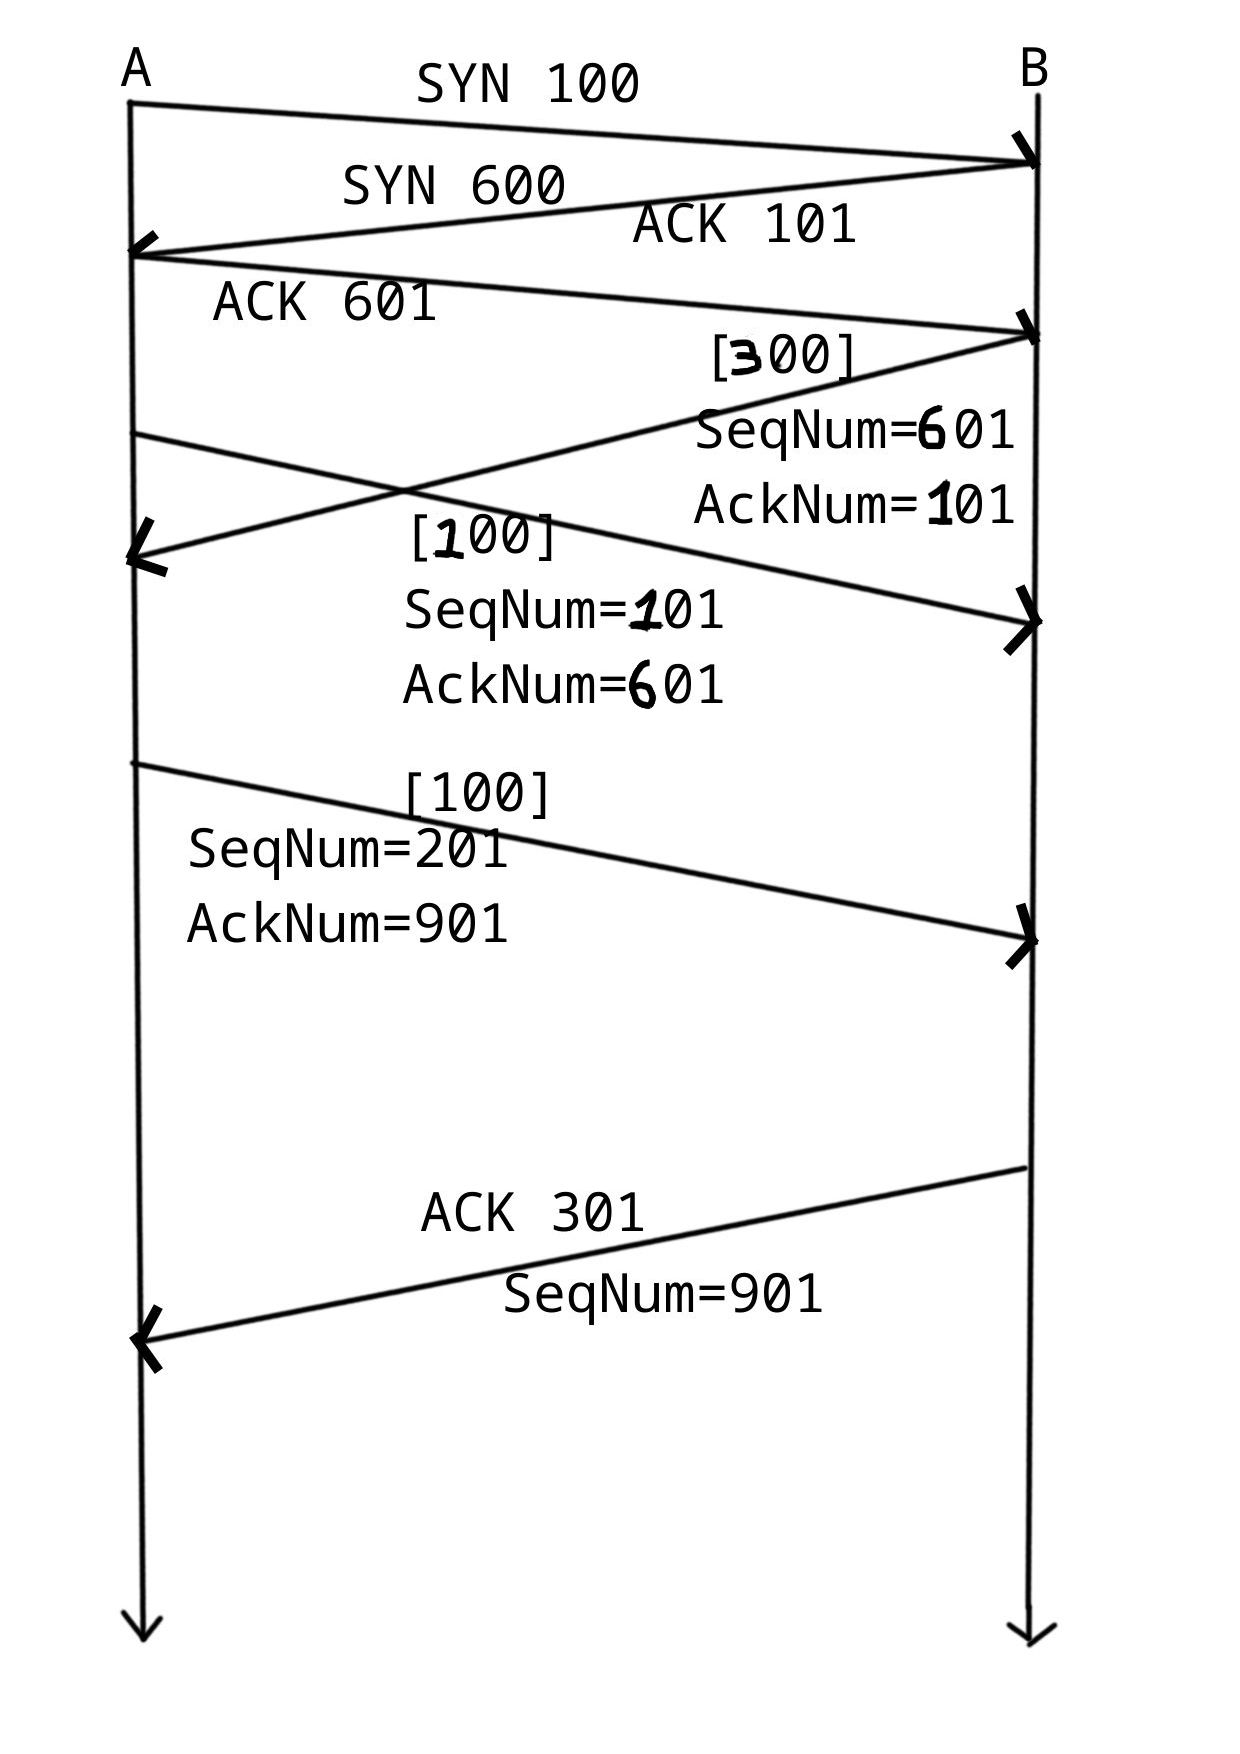
\includegraphics[width=\linewidth,height=0.75\textheight]{TDs/schemas/chronogramme_echange.jpg}
  \caption{Chronogramme d'échange entre A et B}
  \label{fig:chronogramme1}
\end{figure}

Si le premier segment de données de A se perds, alors l'AckNum de B contiendra 100 de moins que le SeqNum de A, ce qui pousse B à envoyer un
ACK pour indiquer qu'il manque le packet à partir de 101.

\subsubsection{Question 3}

Résumé du chronogramme:
\begin{itemize}
  \item Envoie d'abord de 'a', attente d'ACK/tampon plein.
  \item Envoie "bcde", attende d'ACK/tampon plein.
  \item Envoie "fghi".
\end{itemize}

Si la connection est de type "TelNet full duplex", les observations sont les mêmes.

\subsubsection{Question 5}

Elle va grandir exponentiellement jusqu'à la moitié de la taille de lafenêtre avant le crash, 9 Ko dans ce cas.\\
Elle sera donc de la taille du seuil au bout de 4 transmission acquitées, si tout se passe bien.\\
Après le seuil, au lieu de faire une croissance exponentielle, on incrémente seulement la quantité d'octets qui passent.
